%!TEX root =  main.tex
\section{Other considerations}
\label{sec:considerations}

In this section we present a straightforward generalization of the classic $F$ and $F_1$ to allow other exponents. In Section \ref{subsec:fq} we show that in this generalized class of statistics $F_1$ is indeed optimal. In Section \ref{subsec:params} we discuss the experimental exploration of the full parameter space that guides the formulation of the $F_1$ statistic.

\subsection{Varying the exponent}\label{subsec:fq}
As seen is the previous sections, the change from squaring the differences in the original $F$-test to taking their absolute value with the $F_1$-statistic improved power significantly in the differentially private setting. It is not obvious that switching the exponent from 2 to 1 is optimal --- perhaps some other exponent is superior. An exponent of 0 is clearly horrible, so there must be a local maximum in the power of the statistic for some exponent between 0 and 2.

In order to determine which exponent is in fact optimal, we further generalize the notion of an $F$-test.  We define \sqa and \sqe, which are equivalent to \ssa and \sse except that the summand is raised to the $q^{\text{th}}$ exponent, and we call the resulting statistic $F_q$.  Note that $F_1$ (as defined earlier) is a special case of $F_q$ for $q=1$, and $F_2$ is the standard $F$-statistic.

\begin{definition}[$F_q$] \label{def:Fq} 
Given a database \x with \k groups and \dbsize total entries, define \sqa and \sqe as follows:
%
\begin{equation*}
\sqa(\x) = \sum_{j=1}^k n_j \left\vert \overline{y}_j - \overline{y} \right\vert^q
\end{equation*}
%
\begin{equation*}
\sqe(\x) = \sum_{i=1}^N \left\vert y_i - \overline{y}_{c_i} \right\vert^q
\end{equation*}
%
Then, $F_q$ is defined as
%
\begin{equation*}
F_q(\x) = \frac{\sqa/(\k-1)}{\sqe/(\dbsize-\k)}
\end{equation*}
%
\end{definition}
%%%
We must now create a private approximation of $F_q$ for arbitrary $q$.  To do this, we first bound the sensitivity of the \sqa and \sqe with the following two theorems, the proofs of which can be found in Appendix \ref{sec:fqsensitivity}.
%%%
\begin{theorem}[\sqe Sensitivity] \label{thm:SQEsens} 
The sensitivity of \sqe is bounded above by
\begin{equation*}
2\bigg(\frac{\dbsize}{2}\bigg)^{(1-q)} + 1
\end{equation*}
when $q \in (0,1)$ and
\begin{equation*}
\dbsize - \dbsize\bigg(1-\frac{2}{\dbsize}\bigg)^q +1 
\end{equation*}
when $q\geq 1$. Note that both give an upper bound of 3 when $q=1$.
\end{theorem}


\begin{theorem}[\sqa Sensitivity]\label{thm:SQAsens} The sensitivity of \sqa is bounded above by 
\begin{equation*}
\dbsize\bigg(\frac{3}{\dbsize}\bigg)^q + 1
\end{equation*}
when $q \in (0,1)$ and
\begin{equation*}
\dbsize-\dbsize\bigg(1-\frac{3}{\dbsize}\bigg)^q + 1
\end{equation*}
when $q \geq 1$. Note that both give an upper bound of 4 when $q = 1$.
\end{theorem}


Given these sensitivity bounds, we can calculate a private approximation of $F_q$ for simulated data using the same algorithm as for $F_1$, but with the sensitivities altered according to the choice of $q$.  We can also simulate a reference distribution by adapting Algorithm~\ref{alg:pval}, which was done to construct Figure \ref{fig:fqpower}.  As is clear from these results, in terms of power, the optimal value of $q$ is 1.

We note that in the computation shown in Figure \ref{fig:fqpower}, we don't estimate $\sigma$ using \sqe.  This is because we have not developed an estimator for $\sigma$ that can be computed from \sqe (for $q \ne 1, 2$).  If another value of $q$ had indeed been optimal, the next step would have been to find such an estimator and confirm it was accurate enough to produce acceptable $p$-values.  But since the power cannot possibly improve when switching to an estimated $\sigma$ value, this result is sufficient to show that other values of $q$ need not be considered.


\begin{figure}
\centering
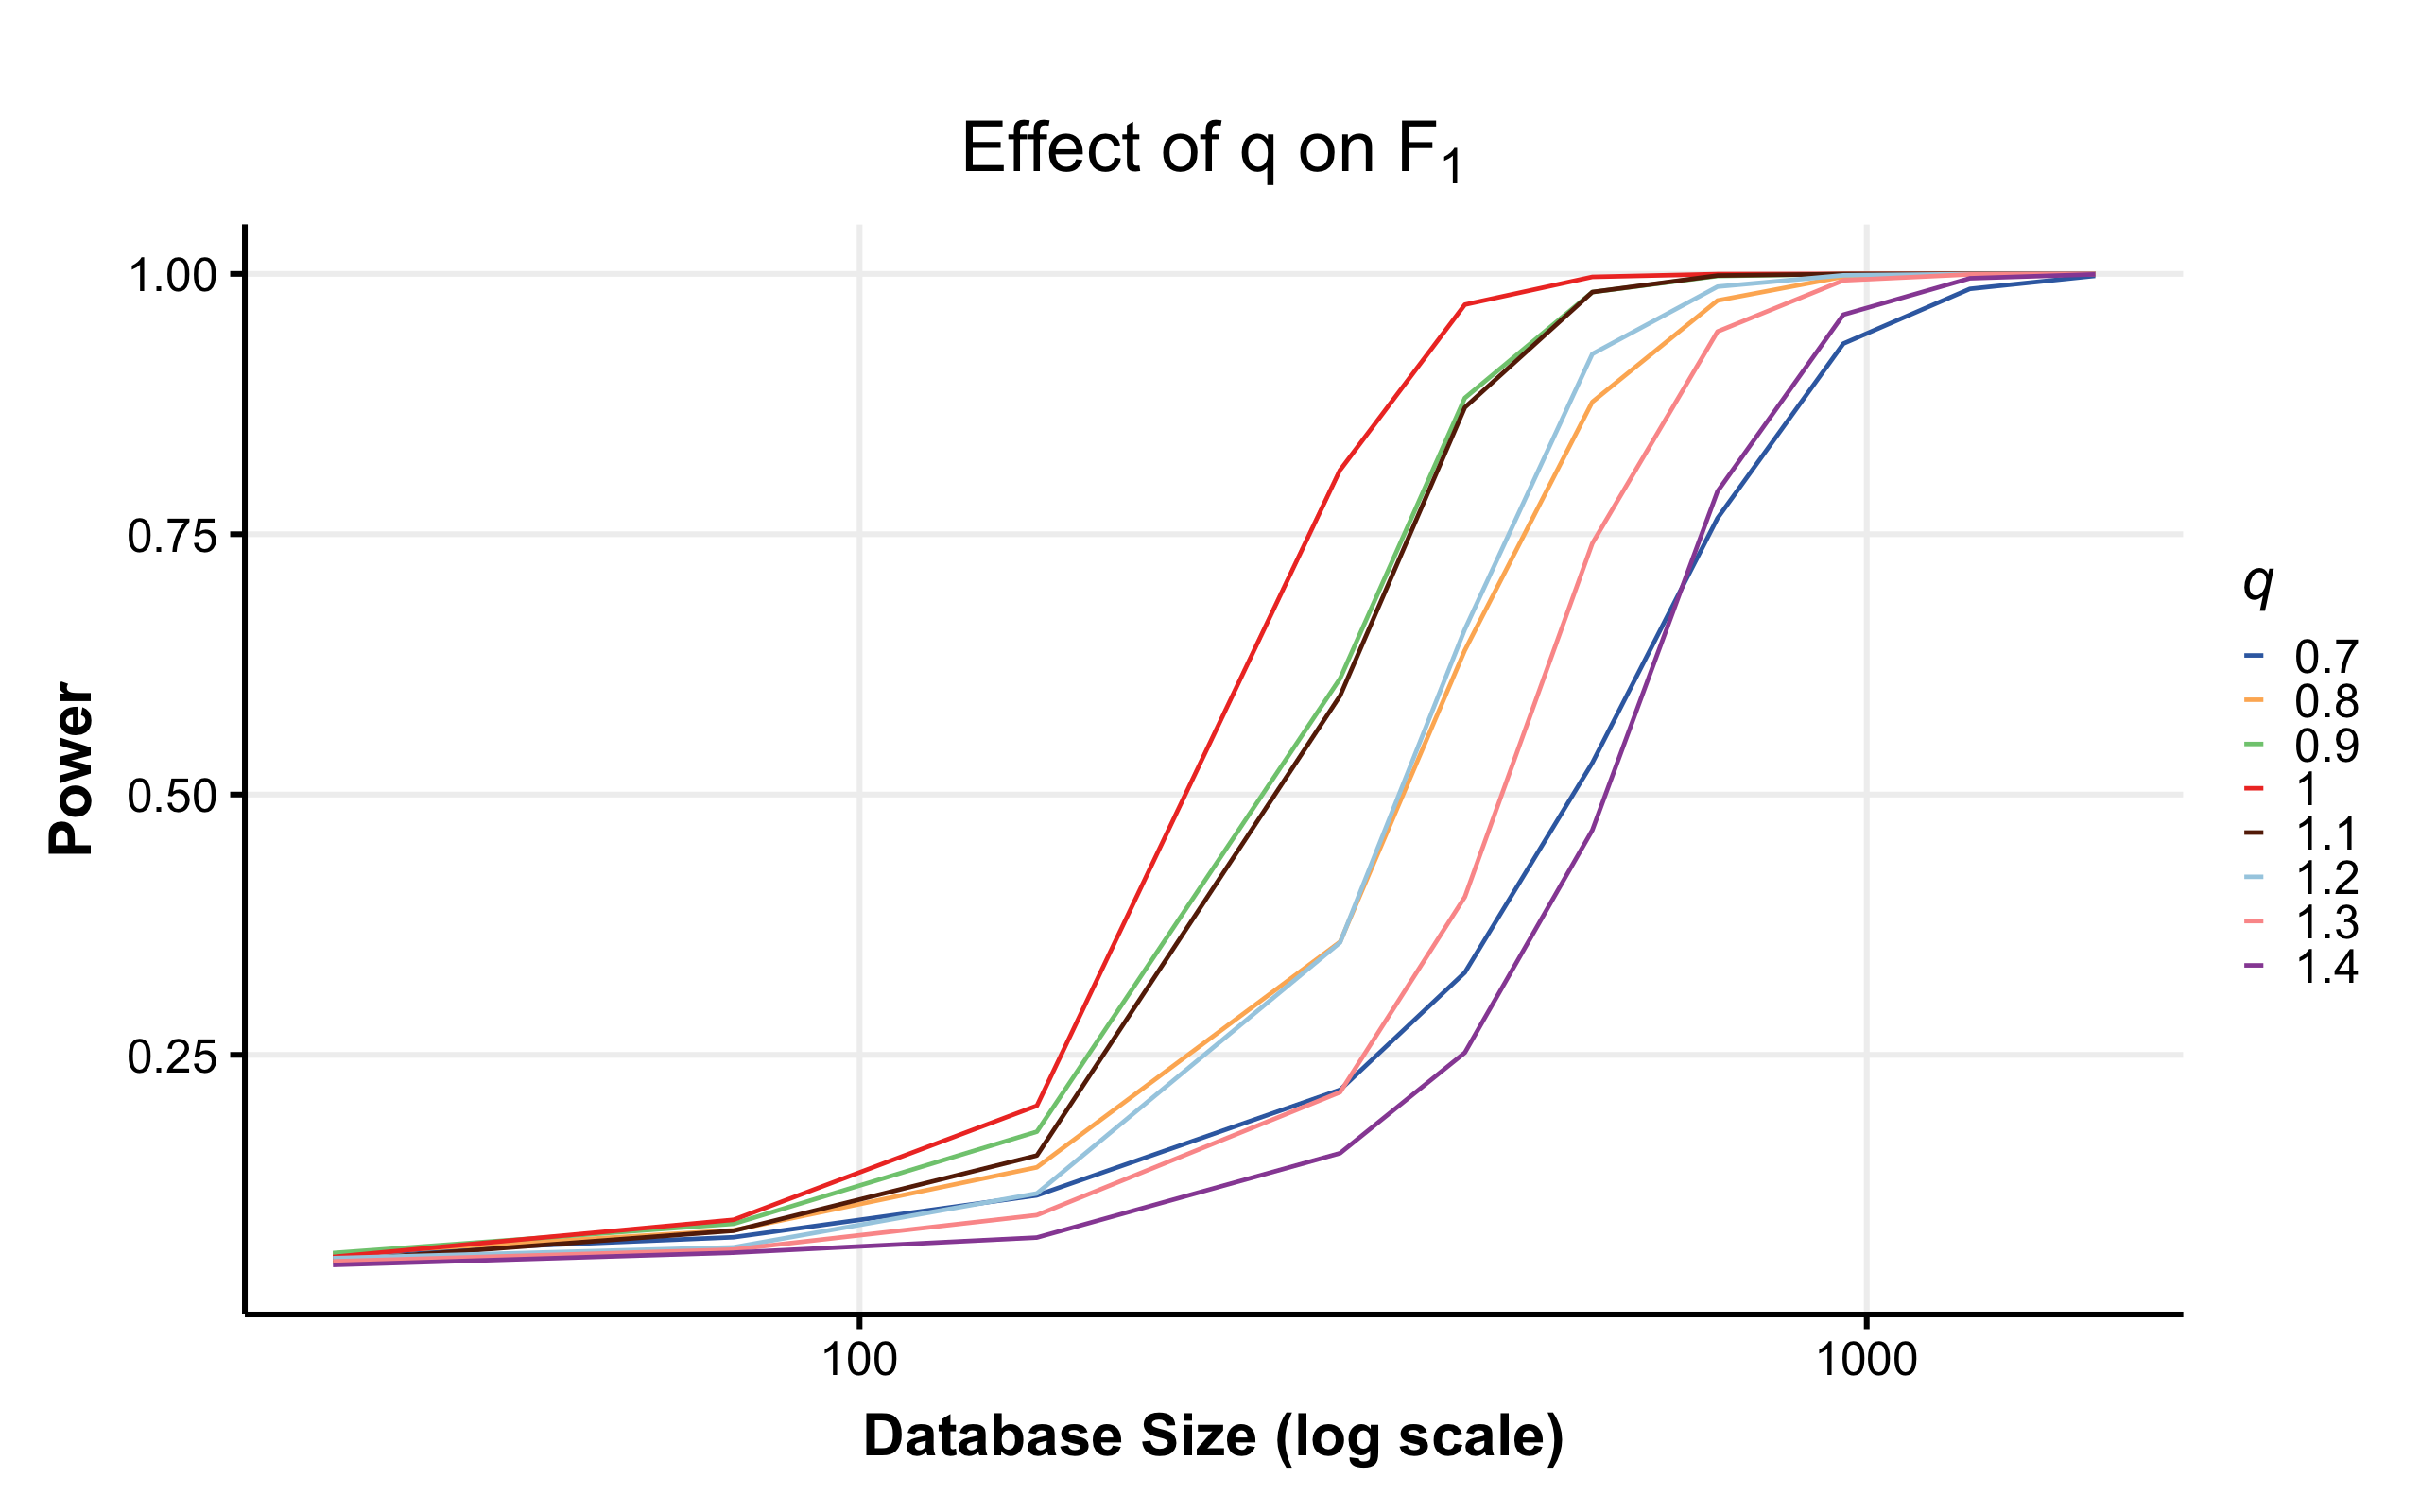
\includegraphics[width=\linewidth]{fq-power.png}
%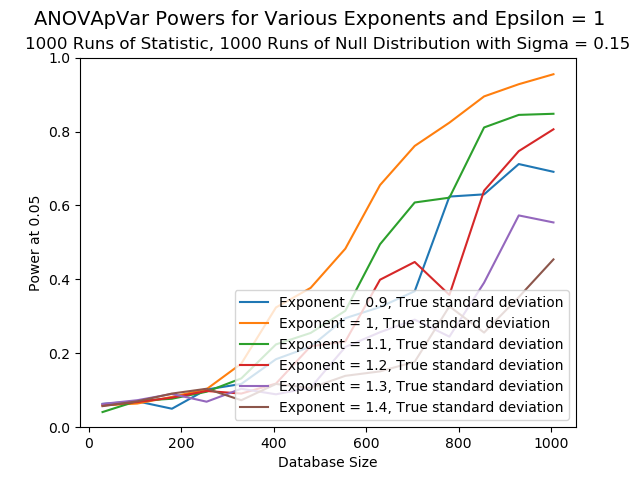
\includegraphics[width=0.8\textwidth,natwidth=610,natheight=642]{Placeholder_manyExponents.png}
\caption{Power curves at varying exponents in a simulation setting where $k = 3$, $\sigma = .15$, and effect size: $1\sigma$. Power is experimentally maximized when $q = 1$.}\label{fig:fqpower}
\end{figure}



\subsection{Parameter tuning}\label{subsec:params}

With the generalization of the $F$-statistic, we add $q$ to the list of parameters that determine the power of a testing procedure. The parameters can be organized as follows:

\vspace{3mm}
\textbf{Data Generation:} $N$, $k$, $\sigma$, effect size \\
\indent\textbf{Private Algorithm:} $\epsilon$, $q$, $\rho$
\vspace{3mm}

The analyst gets to select the parameters corresponding to the private algorithm. While
$\epsilon$ is set based on privacy concerns, $q$ and $\rho$ should be set to 
maximize power, which our work suggest occurs at roughly 1 and 0.7, respectively.
This conclusions is based upon an extensive exploration of the parameter space, 
a selection of which can be found in Appendix~\ref{Sec:AppOptPars}.

The salient feature of these plots is that the choice of $q$ is much more 
consequential than the choice of $\rho$. In the setting where $\epsilon = .1$, 
we found that the result seen in Figure~\ref{Fig:f1-vs-f2} -- a greater than 
10-fold reduction in database size to get equivalent power -- holds across a range
of difference data generation parameters.

By contrast, the effect of $\rho$ on power is much smaller; the database size
reduction is closer to 1.1- or 1.2-fold when moving from $\rho = .5$ to $\rho = .7$
when $\epsilon = .1$.




% \subsection{$G$-statistics}\label{subsec:gq}
% 
% The $F$ statistic (and the entire $F_q$ family of statistics) works by comparing the variation in group means to the within-group variation of individual data points.  We now introduce a class of statistics $G_q$ that do something slightly different.  They instead compare the within-group variation of individual data points to the overall variation between all data points.  If groups have the same mean, the overall variation and the within-group variation should be roughly equal.  On the other hand, if group means are different, then one would expect overall variation to be higher than within-group variation.
% 
% As with the $F$, we can measure this variation using any distance metric and we allow the choice of an arbitrary exponent $q$ here as well.  The formal definition of this statistic follows.
% 


%One of the main pieces of information we must estimate in all of our tests is the standard deviation of the database. For the $F_1$-statistic, this was estimated using $\widehat{\se}$.  In this section we present an alternative approach that proposes a new class of statistics, which we will call $G$-statistics, that feature a direct estimate of the standard deviation.

%We began by modifying the original $F_2$-statistic\ab{what is the $F_2$ statistic?} to compute the total database variance instead of the \ssa. The \ssa measures the amount of variance between groups, so the total database variance seems like a reasonable proxy for the \ssa.

%After the initial modification of using the variance instead of \ssa, we also investigated the same modifications that we made to the $F_2$-statistic, i.e. varying the exponent and the epsilon allocation. The $G$-statistics, which we define below, performed significantly worse than the $F_1$-statistic, with a few exceptions. \ab{we should probably define it first, so readers now what we're talking about, then discuss the riffs.}


% \begin{definition}[$G_q$-statistic] \label{def:Gq} Given a database \x with $k$ groups and $n_j$ entries in the $j$-th group, the $\var_q$ calculation is defined as follows
% \begin{equation*}
% \var_q = \sum_{i=1}^N \lvert y_{i} - \overline{y} \rvert^q.
% \end{equation*}
% Where $q$ is a positive real number. The \sqe is as was defined previously in Definition~\ref{def:Fq}.
% 
% Now, we define the $G_q$-statistic,
% \begin{equation*}
% G_q = \frac{\var_q/(\k-1)}{\sqe/(\dbsize-\k)}
% \end{equation*}
% \end{definition}
% 
% 
% Now that we have defined a new family of statistics, what remains is to repeat everything that was done for the $F_q$ family of statistics.  For simplicity, we leave the details to Appendix \ref{sec:Gapp}, but we summarize the results below.
% 
% First we experimentally optimize the choice of $q$, exactly as was done for the $F_q$ family, and we find the same result --- the ideal choice is $q=1$.  We then optimize the privacy budget allocation for $G_1$.  Here we get different results than with the $F_1$ statistic.  We use $\rho=0.4$ as a roughly optimal value, but unlike in the case of $F_1$, the exact value of $\rho$ seems to have almost no effect --- values in the neighborhood of 0.4 result in a similar-enough power level that our experiments were unable to differentiate the results.
% 
% What remains is then to compare $F_1$ and $G_1$, which we do through simulation.  It is hard to intuitively understand why one or the other might be better, but we find that in most cases $F_1$ is superior.  This should not be surprising because the $F$ statistic is the optimal statistic in the public setting, but as we have already seen the optimal statistic in the public setting need not be optimal in the private setting.
% 
% However, we do find one situation where the $G_1$ statistic outperforms $F_1$.  This is in situations where the within-group standard deviation $\sigma$ is very small, but the difference between group means in $H_A$ is very large (many standard deviations).  This makes sense and results from the why $\sigma$ is estimated in the two statistics.  The estimate of $\sigma$ in $F_1$ is based on \se, which estimates the variance within each group.  By contrast, the estimate we use in the $G_1$ test is based on $\var_1$, and it estimates the total variance across all groups.  These two methods are equivalent under the null hypothesis, so both are acceptable and produce valid $p$-values.  But under the sort of $H_A$ described above, the variation across all items is much larger.  This means that negative $\sigma$ estimates are more rare, and the reference distribution is narrower.  As a result, power increases.
% 
% Unfortunately, the $G_1$ statistic has another problem.  Unlike the $F_1$-statistic, the $G_1$-statistic's type I error increases as the group sizes become more skewed and unequal. This raises the concern that $G_1$ will wrongly reject the null hypothesis too often, and thus be unreliable for hypothesis testing. 
% 
% In conclusion, we find that the $G_1$ test statistic is preferable to the $F_1$ statistic if 1) the within-group variance is very low, 2) the difference between groups is very large, and 3) the groups are known to have roughly equal sizes.  This is a very limited situation, and even in this situation the advantage of $G_1$ over $F_1$ is usually not large.  Therefore we feel confident saying that for general use one should default to the $F_1$ described previously. 



